In this conclusive chapter, some of the most salient obtained results
are presented. First, a brief overview of the important tests
developed during the coding stage of the framework are described;
these include complete tests for almost every part or module of the
system. After this, a qualitative analysis of the performance of both
the vision and gripping modules is done; finally, some thoughts about
the overall benefits introduced by this project and the possible
improvements are stated. 

\section{Developed tests and applications}
Each part of the system has been extensively tested before moving to
the next part; here are presented the most important tests and
programs which have been created for the project. 

First, I/O serialization methods have been created for each module;
these are capable of creating and reading text files containing their
own data structures, specified with the YAML format introduced into
sec.~\ref{sec:standards}. Serialization is done in a recursive way, i.e. being
each module capable of reading its own structure, to read the
corresponding data members it is sufficient to use the standard OpenCV
functions, which will in turn call the correct methods of each
member's type. An example of the YAML data produced by
the \pre{Camera} class when saving camera calibration data is given in
app.~\ref{app:yml}, containing the stored parameters for the Kinect
camera used during the tests. 

For camera modelling, two separate applications have been built, which
implement the two algorithms described into
sec.~\ref{sec:camera-calibration}. This separates the calibration
training into two stages, one for calibrating the intrinsic parameters
and one for the extrinsic; this separation is useful as the internal
parameters of a camera can be calibrated once for its whole lifetime,
while the  extrinsic parameters can be quickly recomputed online for
each view, or can be given from known information (e.g. for the
precision camera used into this project, they can be obtained by
knowing the pose of the robotic arm). Experiments have shown that the
program is able to fit both parameters correctly, and in a good
way. The already shown fig.~\ref{fig:extr_alignment}, is a screenshot
taken from the extrinsic calibration software from real-world data. A
special care had to be taken and is useful to know in order to
calibrate the intrinsic parameters of the depth camera: as the only
image source that can be used comes from the reflected speckle pattern
caught by the infrared sensor, speckles are seen neatly by the
infrared camera, which thus provides a very noisy image to the
chessboard recognition algorithm; in order to fix this, it has been
sufficient to fix a piece of very light paper in front of the infrared
sensor while calibrating: in this way, the speckle pattern is blurred
uniformly by the paper and a flat, grayscale image is seen by the sensor.

After calibration, two different test programs can be run to check
for the correct execution of the latter: the first informs the user
about 3D coordinates of clicked points taken from a stream of images of
the camera, while the second uses the 3D reconstruction module to show
the user a 3D point cloud model of the scene the camera's looking at.

Regarding the robot's movement, the main module which works on it uses
the COMAU's C5GOpen libraries to communicate with the robot; the
corresponding test makes the robot move in front of each bin in
rotation, which can be used to check for both correct setup of the
robot and correct configuration of the bins' reference frames.

Numerous programs have been written to debug every part of the
OpenGL rendering engine: each of these can render mostly a single
mesh in different parts of the scene, the main difference between them
being how the model is read and how the pose is generated: for
example, one program can draw a single mesh -- which is used to test
the rendering engine itself -- in sparse poses into the global
coordinates, while another one can draw the same meshes by parsing 
the folders used to describe the objects' set in order to test the
abstraction layer going from the mesh concept to the more practical
\emph{item} concept.

The vision system is completed with the full training and recognition
test programs, which are evaluated in detail into
sec.~\ref{sec:result-tests}.

Regarding the gripping systems, in turn, many programs have been
created. The first set of them can test the shape generation: when
writing these, shape visualization libraries have been created which
complete the framework as a debugging API; another set of tests
computes several shapes' intersection and outputs the corresponding
volumes: the scenes it acts on are based onto ad-hoc CAD models, and
these can be used to verify that the computed volumes are actually
correct. Finally, a third set of tools tests the grasp generation
algorithm, by creating a random virtual scene and trying to find the best
grasp for several input items, and the overall operative strategy of
the proposed solution, by emulating inputs from the lower-level
modules and performing a simulation of the order in which the objects
are taken.

\section{Performance analysis of the implemented solution} \label{sec:result-tests}
Here follows a qualitative analysis of the behaviour of the main parts
of the solution which are found at the upper level of abstraction,
with focus of the training process, recognition pipeline, and pose
generation algorithm.

\subsection{Analysis of the Line-MOD training process}
The training stage explained in sec.~\ref{sec:training} is performed
by a standalone program, which reads models from an empty training
folder, containing only YAML files describing the model properties
(such as name and meshes), and creates for each a set of views of the
object itself, from which the final set of Line-MOD templates is
extracted. This is finally stored back into the training folder and
will be used by the subsequent algorithms for model recognition.
Three main factors have been found to influence heavily the performance of this algorithm: the used
detector/trainer, the number of viewpoints, and the accuracy of the
render. Each of this sets a speed/performance tradeoff which can
increase the training time but allow a better success rate while
recognizing.

The first element to take into consideration is the number of points
on which the templates are built. A higher number of points will lead
to a proportionally higher computational cost, but will increase the
chance that a grabbed view of a model corresponds to a known view. It
is suggested in \cite{linemod-paper} that a good number of these
for a working recognition system is about 2000. However, this result
is obtained into an experiment in which the rough position of the
object is known a priori, having full vertical rotation range, but
only 90° tilt rotation and half of the possible in-plane
rotations. This is not acceptable for the solution of this problem,
especially because of the presence of many cuboidal objects, which can
be found lying in every orientation; thus, full coverage of the view
sphere and of in-plane rotations is needed upon every dimension. Also, the Kinect used to perform recognition must
stand quite away from the object and these are not big at all, being
mainly in the range $10\sim 20\unit{cm}$ for each dimension. Thus, experiments have shown
that a good candidate for the templates' number is in the range
$15000\sim 20000$; this surely slows down the overall recognition speed,
but this is hardly influential with respect to the other algorithms:
instead, having full coverage of the viewpoints has been noticed to
increase a lot the success rate, especially due to the small distance
in radius between each trained viewpoints' sphere. The counterpart for
this is a higher number of false positives, which have to be filtered
from the hue filtering algorithm.

The choice of the detector used by the training and recognition
algorithm for each model is important too; two detectors have been
implemented for the Line-MOD algorithm; the first is based on the
original implementation found in \cite{linemod-paper}, while the
second is a modified version of this, in which colour gradient
features are not analysed only onto the object's boundaries, but into
the whole template image. Again, this choice conditions both the
training speed, the recognition rate and the false positive one. In
particular, the training and recognition speeds decrease a lot when
the full analysis of the image is done, but the false positive rate is
highly decreased. The recognition rate, for the average case, is not
increased deeply by the use of this system, which is thus rather
avoidable for most of the objects. The case in which the full image
matching performs decisively better is in the recognition of weakly
textured objects, with trivial shape factors, and poorly saturated
colours. In such cases, the image gradient found on borders is flat,
due to the low saturation of colours, and thus informations coming
from the internal part of the object (text, images, etc.) can be vital
for the proper operation of the algorithm, although at the cost of
higher execution times.

Finally, the usage of the improvements on the rendering quality
explained into sec.~\ref{sec:antialiasing} help mainly by removing the noise on
the border of the renders; this increases the computation time
needed by the training algorithm, but has no impact at all on the
recognition speed; at the same time, the recognition rate is slightly
increased, and this improvement becomes important in the case of small
or very far objects: in this case, the distortion brought by the
missing antialiasing in renders is no more negligible with respect to
the size of the templates themselves. This makes turning on full
antialiasing a good choice for most of the applications.

\subsection{Recognition performance of the Line-MOD pipeline}
A set of tests have been done onto the Line-MOD pipeline in order to
establish how it performs well for many different types of objects,
including the ones from the object set of the Amazon Picking Challenge
and some more taken as a reference. Results show an overall good
performance, especially is the minimum recognition threshold is kept
some points below $100\%$ (in these experiments, we used $97\%$ as a
starting threshold, which can be lowered if needed by the pipeline as
explained in sec.~\ref{sec:linemod-pipeline}); in this case, many
false positives arise, which is a problem already observed for the
Line-MOD algorithm in \cite{linemod-pipeline}, and thus justifies the
need for the hue-based filtering used as a second step of the
pipeline. However, this last filter is able to correctly filter out
most of the false positives correctly, and the seldom remaining ones
are usually dropped into the last part of the pipeline by the low
convergence threshold of the ICP algorithm. The hue-based filter
has been however found quite critical to tune for proper operation: in
particular, it is important to tune the two thresholds for considering
the pixels to be white or black in order to fit well the general
illumination conditions of the experiment.

From the experiments, it has been observed that the object set can be
divided approximately into four classes: the first is the case in which
objects have bright colour, medium to big dimensions, and a
non-standard shape, such as the bottle brush shown in the first part
of fig.~\ref{fig:apc-object-sets}; the second and most populated one correspond to those
objects which have standard cuboidal shapes, but still maintain
well-saturated textures with patterns such as colour changes on the
contour, like the board eraser of the same figure; these are mainly
recognized correctly, but the false positive rate is increased
significantly as many views don't bring sufficient depth information,
being their faces seen as planes by the depth sensor; however, as
explained before both the hue filter and the ICP alignment steps are
usually able to drop all the false positives without relevant
problems.

The third object set is exemplified by the self-stick notes stack:
these object have small dimensions and low-saturation foreground
colours, such as bright yellow or grey. In this case, the background
may become problematic, and a good tuning of the hue filter becomes
necessary to avoid it accept false positives corresponding to portion
of floor or furniture, as they often have low-saturated colours too
and thus the contrast is minimal. For these objects, a solution which
has been seen to improve a lot the performance is the use of the
full-image detector instead of the default one: this makes it possible
to recognize patterns, usually in the form of a logo, which are
usually present on every everyday item.

Finally, the last -- and most problematic -- set of object is the one,
like the last one of fig.~\ref{fig:apc-object-sets}, which have big,
flat surfaces, with dark, low-saturated colours and low-contrast
textures on them. These items are rarely recognized properly by the
detector, as the actual number of features on them is quite low and,
being the feature themselves very weak, nondeterministic, especially
due to the black background which impacts the gradient computation and
adds noise to the depth measurements. For these objects, it would be
appropriate to exploit the modularity features of the created
framework to use another, more specific algorithm, for example by
searching the image for low-saturation areas and fitting a cubical
shape onto them with a variation of the RANSAC algorithm of \cite{ransac}.

\begin{figure}[htbp] 
\centering
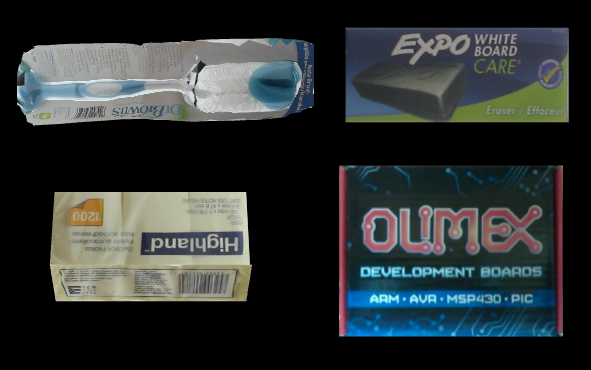
\includegraphics[width=2.5in]{./Graphics/apc-object-sets}
\caption{From the top-left, as rendered by the framework: an object
  with good, smooth shape and good, brilliant colours; an object with
  trivial shape but high-contrast colours, and object with weakly
  saturated colours but high-contrast internal details, an object
  with weakly saturated colours and low-contrast internal details.\label{fig:apc-object-sets}}
\end{figure}

However, the bigger part of the common, daily usage items belong to
one of the first three categories: this makes the Line-MOD based
algorithm a good choice both for the purposes of the Amazon Picking
Challenge and for usage as the default recognition pipeline of the
framework.

\section{Comments on the gripping module}
The gripping module is the only one which has been built essentially from scratch;
this has been due to the extreme fragmentation in libraries and
frameworks regarding this topic; as such, it is also the one which is
most in beta stage. However, the obtained results look promising:
first and foremost, the best grasping pose is correctly generated for
every scene for which the system has been tested. In particular, the
algorithm used for pose constraining succeeds in forcing the gripper to
an arbitrary position without making it assume unnatural poses, which
is particularly important for a small robotic arm such as the COMAU's
Racer999 used into this project.
After tuning the parameters used by each heuristic, it can be seen how
the computational performance of the algorithm is acceptable for the
specifications of the problem, running in the range of few tenth of
precise intersection computations per second on compound
scenes. Whether not optimal, this can, and likely will, be easily
improved by adding further heuristic to each shape: in particular,
some trivial heuristics such as cuboid intersection's skipping have
still not been implemented, and are easy to. This will for sure
improve the performance, and especially it will flatten the currently
high variance in computation cost, which, for example, currently is
$O(1)$ for any sphere-to-sphere intersection and $O(l^2)$ in the
average cuboid-to-cuboid intersection.

Another essential optimization which can easily improve the
performance of this algorithm is the use of multithreading for
computations, as they are mostly independent from each other into the
intersection module. This has been made trivial to do due to the
recent support of every modern system to the C++11 specification,
which provides the \pre{std::async} abstraction for asynchronous computations.

Some tests driven by trial-and-error have shown that it is easy for a
non-skilled operator to correctly implement model files describing the
desired training for picking poses, due to the easy-to-use pose
generation and constraining APIs described in
sec.~\ref{sec:pose-generation}. This is an obvious advantage, and
hopefully will help any future user of the system to approach it
without difficulty, leaving anyway to him the faculty of digging and
modifying the framework's behaviour at any abstraction level without
the need of modifying the codebase of the framework itself.

\section{Conclusions}
The completed project manages to provide both a complete vision and
grasping solution, and more importantly a base over which new gripping
systems can be implemented easily. Although into its initial
development stages with respect to the breadth of the topic which it
tries to fit into, and although improvable for sure, it has an overall
discrete performance if compared to 
state-of-the-art projects that cover the same topics, mainly due to the usage of
many of them in form of software libraries. However, differently from
them, the main improvement that this project brings to the robotics
field is the capability to bring all of these different libraries to
share an overall coherent structure, to completely inhibit fragmentation between
different modules, and more in general to let a future developer
structure in a more efficient and safe way its projects. The total
portability of the system to different software and hardware
platforms, mainly due to the use of free and open source software, and
to the total absence of variation over well-established standards,
combined with the full modularity of the system, will
make the framework easy to maintain, to expand, and to use. A good
starting point for the future improvement of the system would be its
integration with the \emph{Robot Operating System (\emph{ROS})}, which
has become a de-facto standard in recent years, which excellent
support for complex robotics applications; this would help it improve
its internal coherence between its software stacks, which is one of
the fields ROS currently misses the most.

Hopefully, these factors will let future versions of this software play an
important role into the next iterations of the Amazon Picking
Challenge and into the robotics research world in general, in order to help
automated robotic systems find a bigger space into everyday life's applications.
